\documentclass[10pt, xcolor=dvipsnames]{beamer}
\usepackage{kotex}
\usepackage{commath}
\usepackage{multirow}
\usepackage{multicol}
\usepackage{arydshln} % Include this package
\usepackage{bbding}

\usepackage{tikz}
\usepackage{tikz-cd}
\usetikzlibrary{math} % for calculations
\usetikzlibrary{shapes, arrows.meta, positioning, shadows}
\usetikzlibrary{arrows,shapes.geometric}  % Optional, based on your needs
\usetikzlibrary{3d, calc}
\usetikzlibrary{matrix, positioning, arrows.meta, shapes.multipart, chains}
\usetikzlibrary{decorations.pathreplacing,calligraphy}
\usetheme[progressbar=frametitle]{metropolis}
\usepackage{appendixnumberbeamer}

\usepackage{adjustbox}
\usepackage{booktabs}
\usepackage[scale=2]{ccicons}

\usepackage{tcolorbox}

\usepackage{pgfplots}
\usepgfplotslibrary{fillbetween}
\pgfplotsset{compat=1.15}
\usepgfplotslibrary{dateplot}

\usepackage{xspace}
\newcommand{\themename}{\textbf{\textsc{metropolis}}\xspace}

\usepackage[linesnumbered,ruled]{algorithm2e}
\usepackage{algpseudocode}
\usepackage{setspace}
\SetKwComment{Comment}{/* }{ */}
\SetKwProg{Fn}{Function}{:}{end}
\SetKw{End}{end}
\SetKw{DownTo}{downto}

% Define a new environment for algorithms without line numbers
\newenvironment{algorithm2}[1][]{
	% Save the current state of the algorithm counter
	\newcounter{tempCounter}
	\setcounter{tempCounter}{\value{algocf}}
	% Redefine the algorithm numbering (remove prefix)
	\renewcommand{\thealgocf}{}
	\begin{algorithm}
	}{
	\end{algorithm}
	% Restore the algorithm counter state
	\setcounter{algocf}{\value{tempCounter}}
}

\usepackage{xcolor}   % Required for specifying colors

\usepackage{listings} %Code
\renewcommand{\lstlistingname}{Code}%
\definecolor{keyword}{RGB}{255, 0, 0}
\definecolor{identifier}{RGB}{0, 0, 255}
\definecolor{comment}{RGB}{0, 128, 0}
\definecolor{string}{RGB}{163, 21, 21}

\lstdefinestyle{c}{
	language=C,
	basicstyle=\ttfamily\small,
	keywordstyle=\color{keyword},
	identifierstyle=\color{identifier},
	commentstyle=\color{comment}\itshape,
	stringstyle=\color{string},
	showstringspaces=false,
	%	numberstyle=\tiny\color{gray},
	%	numbersep=5pt,
	frame=single,
	tabsize=4,
	captionpos=b,
	breaklines=true,
	breakatwhitespace=true,
	%	numbers=left
}

\definecolor{backcolor}{HTML}{FAFAFA}
\lstdefinestyle{ocaml}{
	language=[Objective]Caml,
	basicstyle=\ttfamily\bfseries\footnotesize,
	keywordstyle=\color{blue}\bfseries,
	commentstyle=\color{gray}\itshape,
	stringstyle=\color{orange}\bfseries,
	numberstyle=\tiny\color{purple},
	identifierstyle=\color{teal},
	emphstyle=\color{red}\bfseries,
	backgroundcolor=\color{backcolor},
	frame=single,
	rulecolor=\color{black},
	frameround=tttt,
	numbers=left,
	numbersep=10pt,
	showspaces=false,
	showstringspaces=false,
	breaklines=true,
	breakatwhitespace=true,
	tabsize=2,
	captionpos=b,
	literate={->}{{$\rightarrow$}}1
	{<-}{{$\leftarrow$}}1
	{=>}{{$\Rightarrow$}}1
	{|->}{{$\mapsto$}}1
	{>>}{{$\gg$}}1
	{<<}{{$\ll$}}1
}

\definecolor{commentColor}{rgb}{0.25,0.5,0.35}
\definecolor{stringColor}{rgb}{0.5,0.1,0.5}
\definecolor{vsCodeRed}{HTML}{E06C6A}
\definecolor{vsCodeBlue}{HTML}{3986E9}
\definecolor{CLIGreen}{HTML}{87D368}
\definecolor{rustBuild}{HTML}{A5BE5D}
\definecolor{rustBack}{HTML}{282C34}
\lstdefinestyle{zsh}{
	language=bash,                  % Set the language to bash (closest to Zsh)
	backgroundcolor=\color{rustBack},
	commentstyle=\color{rustBuild}\ttfamily,
	keywordstyle=\color{rustBuild}\bfseries,
	stringstyle=\color{stringColor!70!white}\ttfamily,
	keywordstyle=[2]{\bfseries\color{rustBuild}},
	keywordstyle=[3]{\bfseries\color{CLIGreen}},
	showspaces=false,               % Don't show spaces as underscores
	showstringspaces=false,         % Don't highlight spaces in strings
	breaklines=true,                % Automatic line breaking
	frame=none,                     % No frame around the code
	basicstyle=\ttfamily\color{white}, % White basic text color for contrast
	extendedchars=true,             % Allow extended characters
	captionpos=b,                   % Caption-position at bottom
	escapeinside={\%*}{*)},         % Allow LaTeX inside your code
	morekeywords={echo,ls,cd,pwd,exit,clear,man,unalias,zsh,source}, % Add more keywords
	upquote=true,                   % Ensure straight quotes are used
	literate=
	{\$}{{\textcolor{vsCodeRed}{$\boldsymbol{\$}$}}}1
	{>}{{\textcolor{CLIGreen}{$\boldsymbol{>}$}}}1
	{<}{{\textcolor{CLIGreen}{$\boldsymbol{<}$}}}1
	{@}{{\textcolor{vsCodeRed}{@}}}1
	{~}{{\textcolor{vsCodeRed}{$\boldsymbol{\sim}$}}}1
	{:}{{\textcolor{rustBuild}{:}}}1,
	%		{:}{{\textcolor{red}{:}}}1
	%		{~}{{\textcolor{red}{\textasciitilde}}}1 % Color certain characters
	%		{├}{{\textbrokenbar}}1  % Replace ├ with \textbrokenbar
	%		{─}{{\textendash}}1     % Replace ─ with \textendash
	%		{└}{{`}}1,              % Replace └ with `
	morekeywords=[2]{cryptol, load, prove, ocaml},
	morekeywords=[3]{Main}
}

\usepackage{amsthm, amsmath}


\newcommand{\cyclic}[1]{\langle #1 \rangle}
\newcommand{\uniform}{\overset{\$}{\leftarrow}}
\newcommand{\N}{\mathbb{N}}
\newcommand{\Z}{\mathbb{Z}}
\newcommand{\Q}{\mathbb{Q}}
\newcommand{\R}{\mathbb{R}}
\newcommand{\C}{\mathbb{C}}
\newcommand{\F}{\mathbb{F}}

\newcommand{\xmark}{\textcolor{red}{\XSolidBrush}}
\newcommand{\vmark}{\textcolor{green!75!black}{\CheckmarkBold}}

\newcommand{\B}{\mathbb{B}}
\newcommand{\true}{\textcolor{red}{\texttt 1}}
\newcommand{\false}{\textcolor{red}{\texttt 0}}
\newcommand{\id}{\textnormal{id}}
\title{\huge\bf \textcolor{obsidian}{Obsidian} for Researchers}
%\subtitle{\textcolor{magenta}{\textbf{Lecture 02. OCaml Programming II}}}
% \date{\today}
\date{}
\author{\large\textcolor{cyan}{\bf Ji, Yong-Hyeon}\\ \\ \small 24. 09. 19 (Thu)}
\institute{\small
	Coding \& Optimization Together (CO2) \\
	Crypto \& Security Engineering Lab (CSE) \\
	Department of Information Security, Cryptology, and Mathematics
}
%\titlegraphic{\hfill\includegraphics[height=1.5cm]{../latex-imagelogo}}

\pgfdeclareimage[height=\paperheight,width=\paperwidth]{myimage}{../latex-image/hexagon_bg}
\usebackgroundtemplate{\tikz\node[opacity=0.5] {\pgfuseimage{myimage}};}

%\setbeamercolor{title}{bg=UniBlue}
\setbeamercolor{frametitle}{bg=obsidian}
%\setbeamercolor{structure}{bg=UniBlue}

\begin{document}
	\maketitle \begin{frame}{}
	\begin{figure}[\centering]
		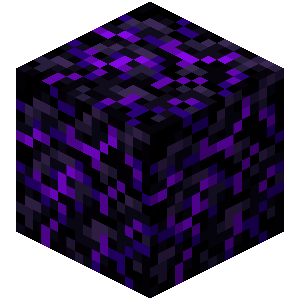
\includegraphics[scale=.5]{../latex-image/obsidian-minecraft}
	\end{figure}
\end{frame}\begin{frame}{}
	\begin{figure}[\centering]
		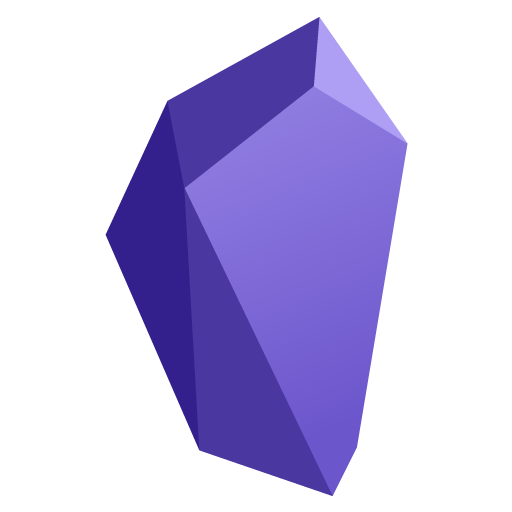
\includegraphics[scale=.3]{../latex-image/obsidian-icon}
	\end{figure}
	\end{frame}
	\begin{frame}{Table of Contents}
		\setbeamertemplate{section in toc}[sections numbered]
		\tableofcontents%[hideallsubsections]
	\end{frame}
	
	\newpage
	\section{What is Obsidian?}
	% Slide 1: What is Obsidian?
	\begin{frame}{What is Obsidian?}
		\textcolor{obsidian}{\bf Obsidian} is a \underline{\textit{Markdown-based note-taking app}} with powerful linking and knowledge management capabilities.\\
		\vspace{0.5cm}
		\textbf{Key Features:}
		\begin{itemize}
			\item Note creation using \textbf{Markdown}.
			\item \textbf{Callouts} to highlight important information within notes.
			\item \textbf{Local} storage (no cloud dependency).
			\item \textbf{Bi-directional linking} between notes.
			\item \textbf{Graph view} to visualize connections.
			\item \textbf{Canvas} to visualize and organize markdown notes.
			\item \textbf{Excalidraw} to draw and link diagrams 
		\end{itemize}
	\end{frame}
	
	\section{Note Creation using Markdown}
	\begin{frame}{Note Creation using Markdown}
		\begin{figure}
			\centering
			\begin{minipage}{.32\textwidth}
				\centering
				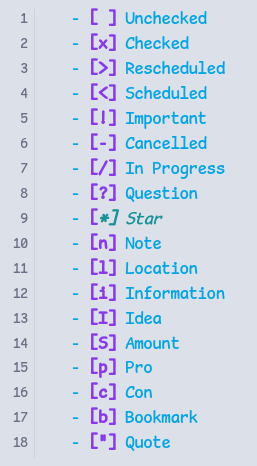
\includegraphics[width=.95\linewidth]{../latex-image/markdown-code1}
			\end{minipage}%
			\begin{minipage}{.32\textwidth}
				\centering
				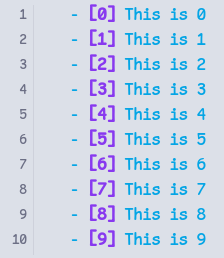
\includegraphics[width=.95\linewidth]{../latex-image/markdown-code2}
			\end{minipage}%
			\begin{minipage}{.32\textwidth}
				\centering
				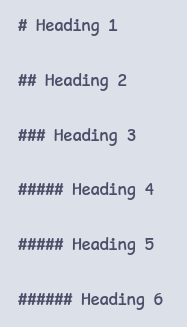
\includegraphics[width=.95\linewidth]{../latex-image/markdown-code3}
			\end{minipage}%
		\end{figure}
	\end{frame}
	\begin{frame}{Note Creation using Markdown}
	\begin{figure}
		\centering
		\begin{minipage}{.32\textwidth}
			\centering
			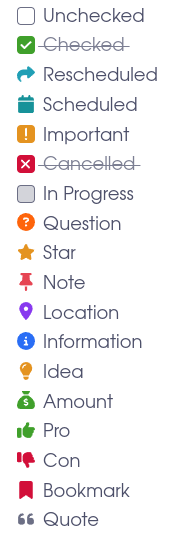
\includegraphics[width=.7\linewidth]{../latex-image/markdown1}
		\end{minipage}%
		\begin{minipage}{.32\textwidth}
			\centering
			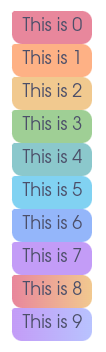
\includegraphics[width=.7\linewidth]{../latex-image/markdown2}
		\end{minipage}%
		\begin{minipage}{.32\textwidth}
			\centering
			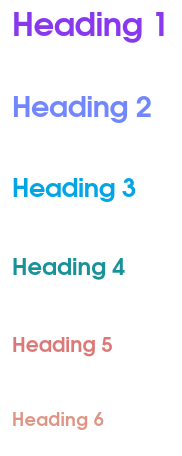
\includegraphics[width=.7\linewidth]{../latex-image/markdown3}
		\end{minipage}%
	\end{figure}
%		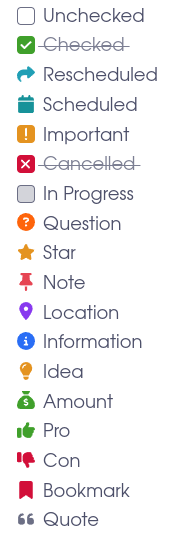
\includegraphics[scale=.2]{../latex-image/markdown1}
%		
%		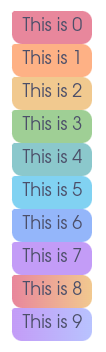
\includegraphics[scale=.2]{../latex-image/markdown2}
%		
%		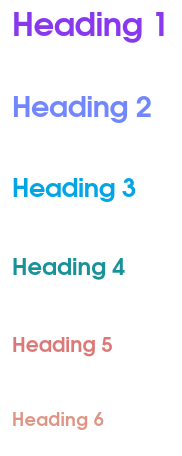
\includegraphics[scale=.2]{../latex-image/markdown3}
	\end{frame}

	\section{Callout}
	\begin{frame}{Callout}\centering
		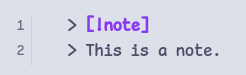
\includegraphics[width=.5\linewidth]{../latex-image/markdown-code4}
	\end{frame}
	\begin{frame}{Callout}\centering
		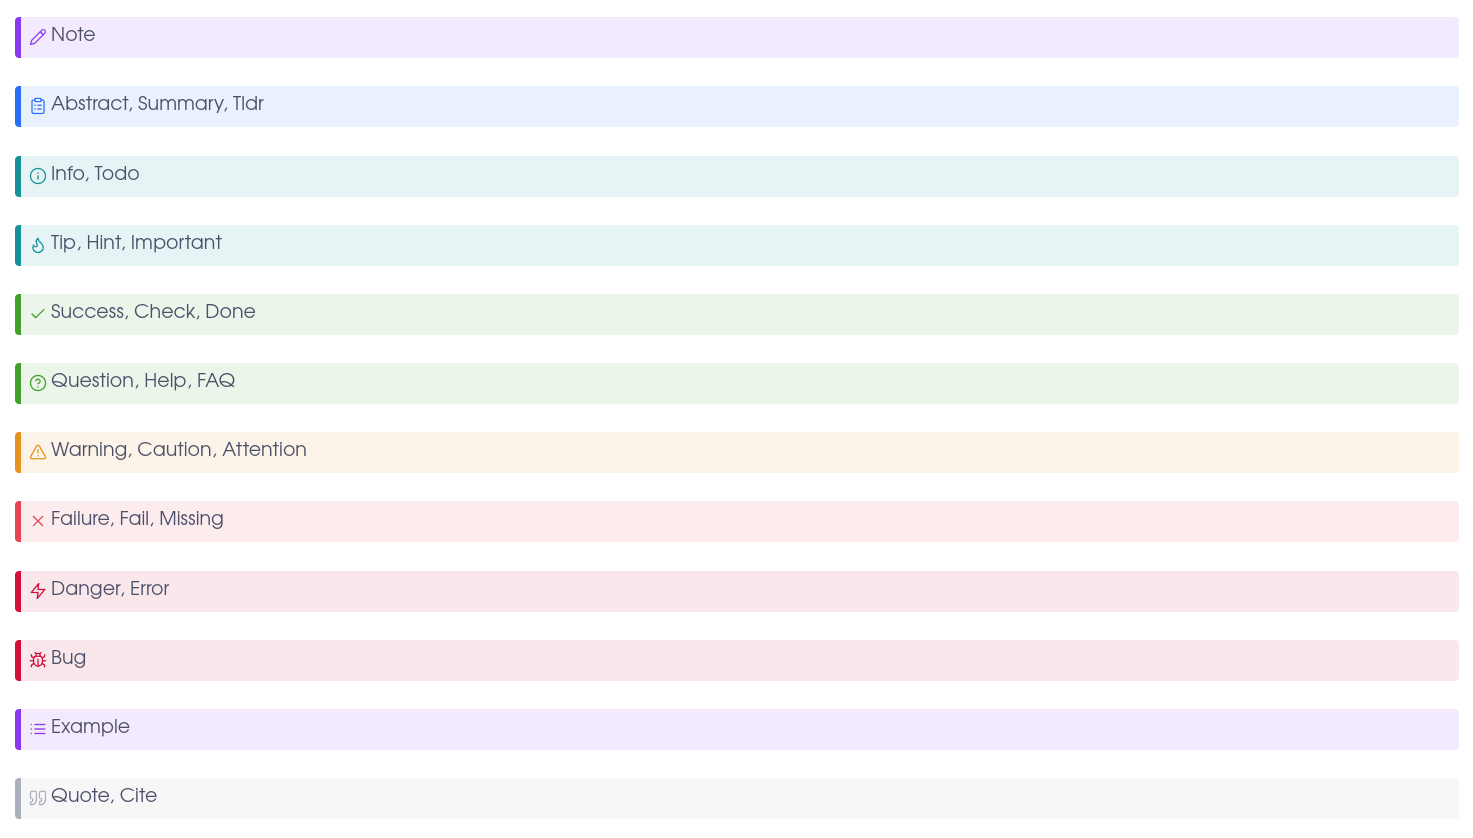
\includegraphics[width=1\linewidth]{../latex-image/callout}
	\end{frame}

	\section{Local Storage}
	\begin{frame}{Local Storage}\centering
		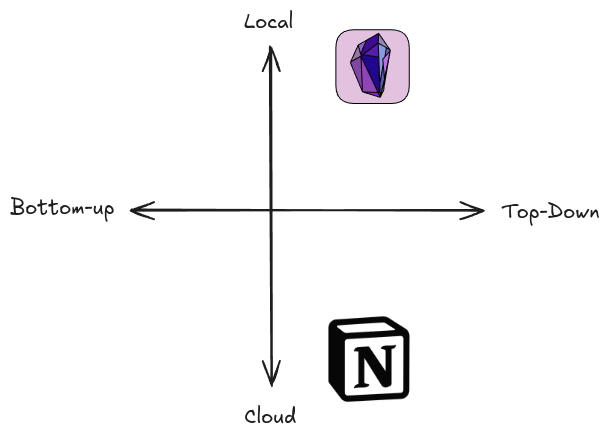
\includegraphics[width=.85\linewidth]{../latex-image/local-storage}
	\end{frame}

	\section{Linking and Graph View}
	\begin{frame}{Bi-directional Linking and Graph View}
		\centering
		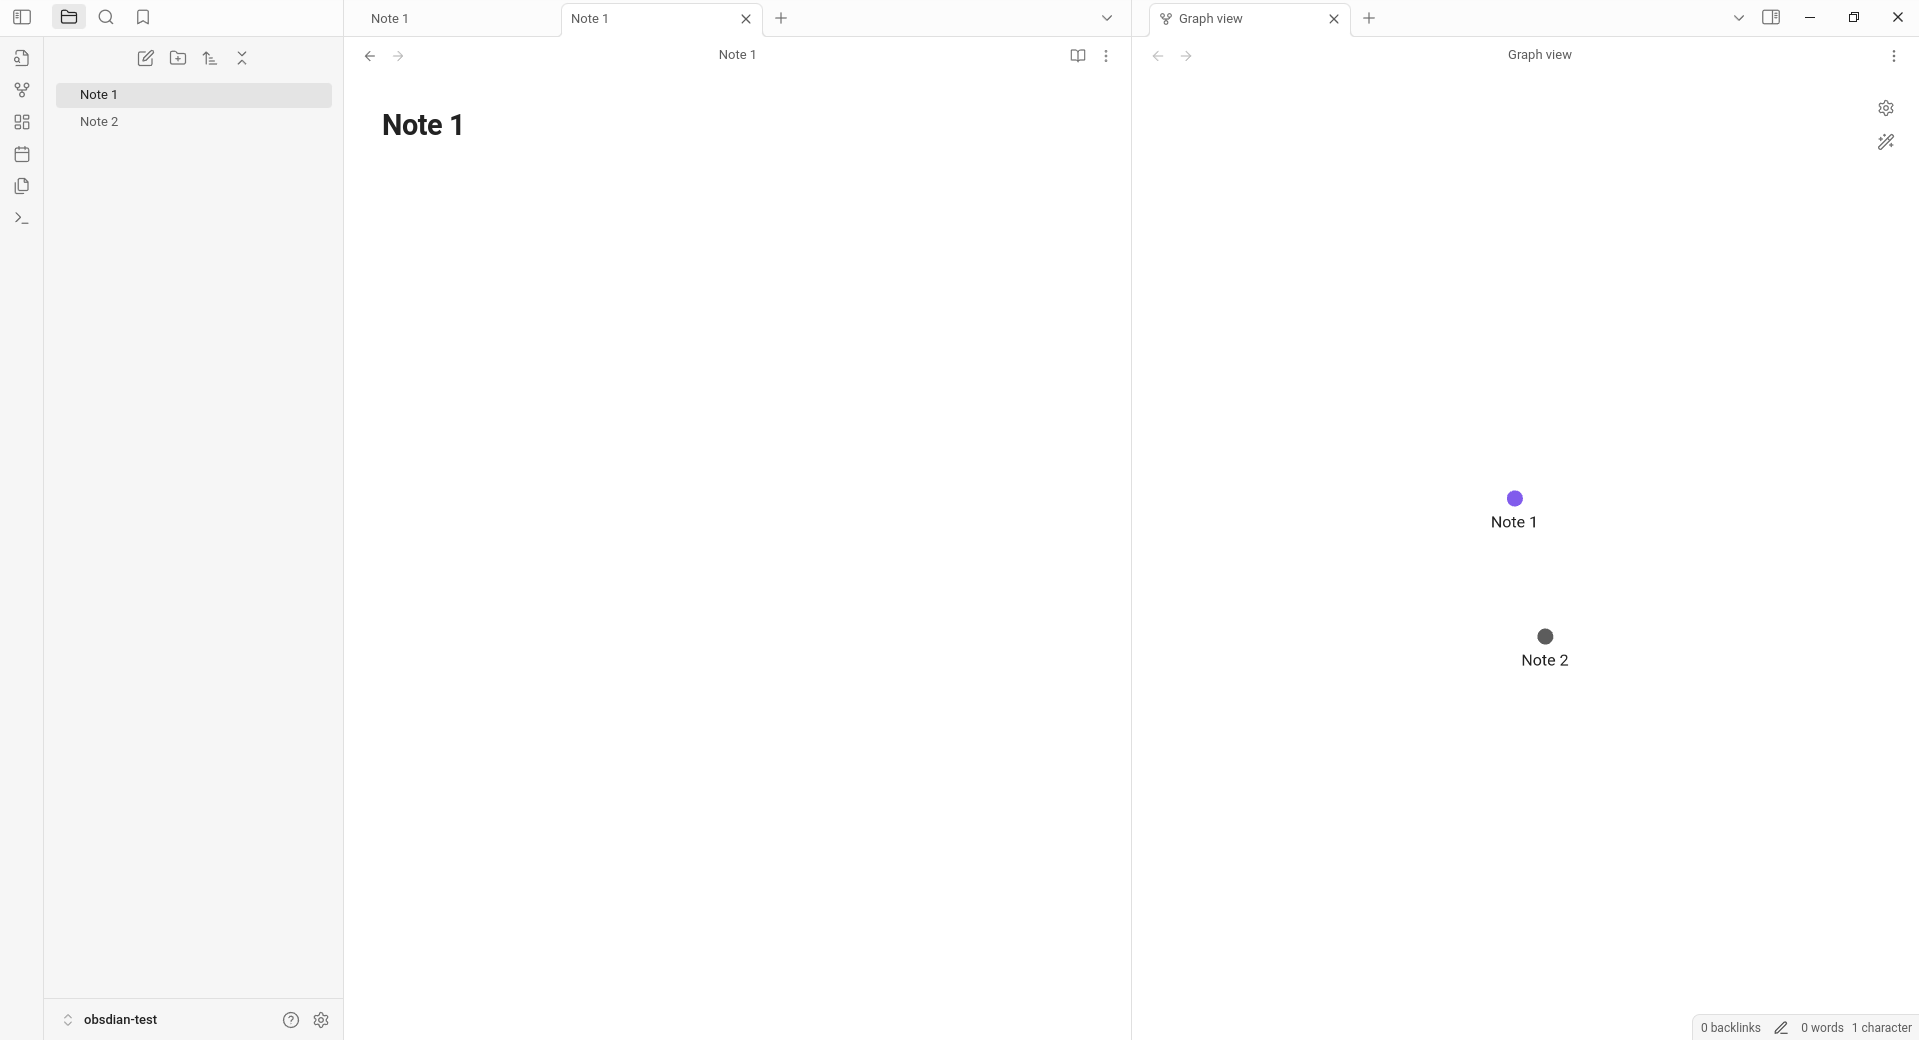
\includegraphics[width=1\linewidth]{../latex-image/linking1}
	\end{frame}
	\begin{frame}{Bi-directional Linking and Graph View}
		\centering
		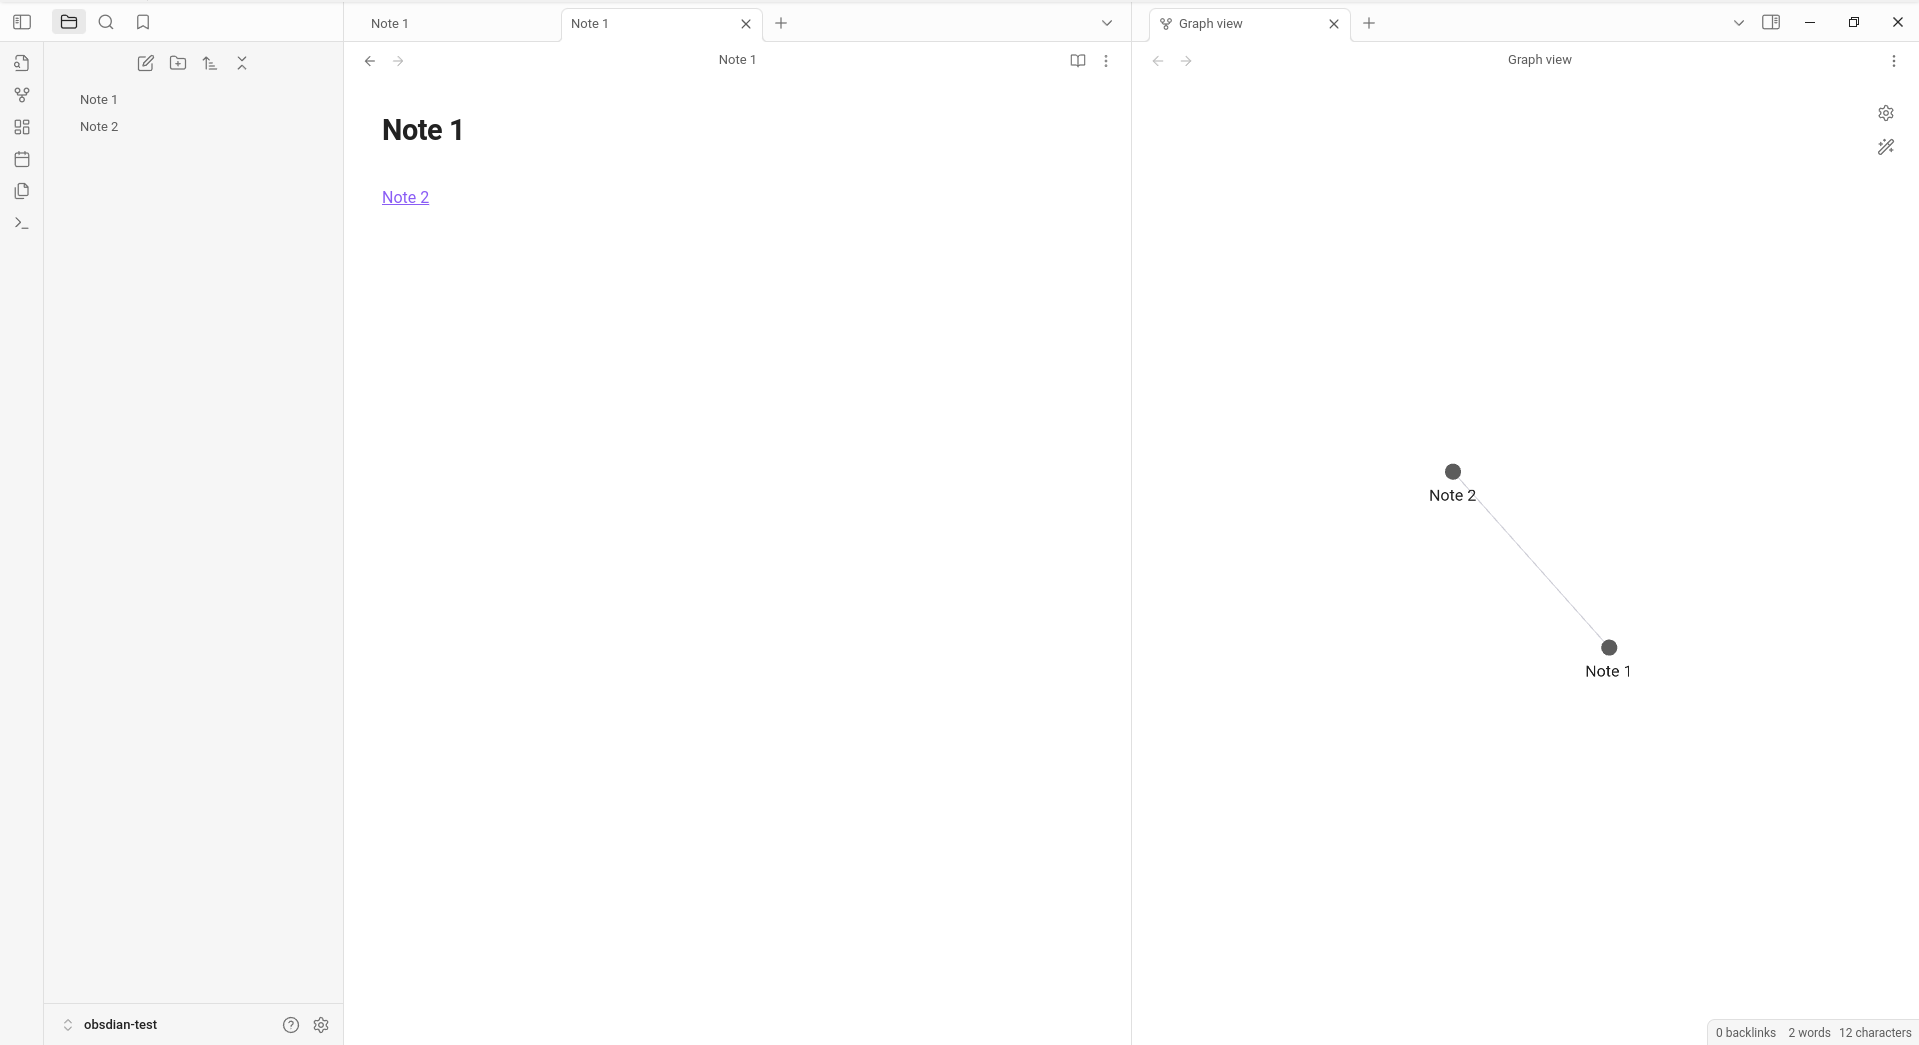
\includegraphics[width=1\linewidth]{../latex-image/linking2}
	\end{frame}
	\begin{frame}{Bi-directional Linking and Graph View}
	\centering
	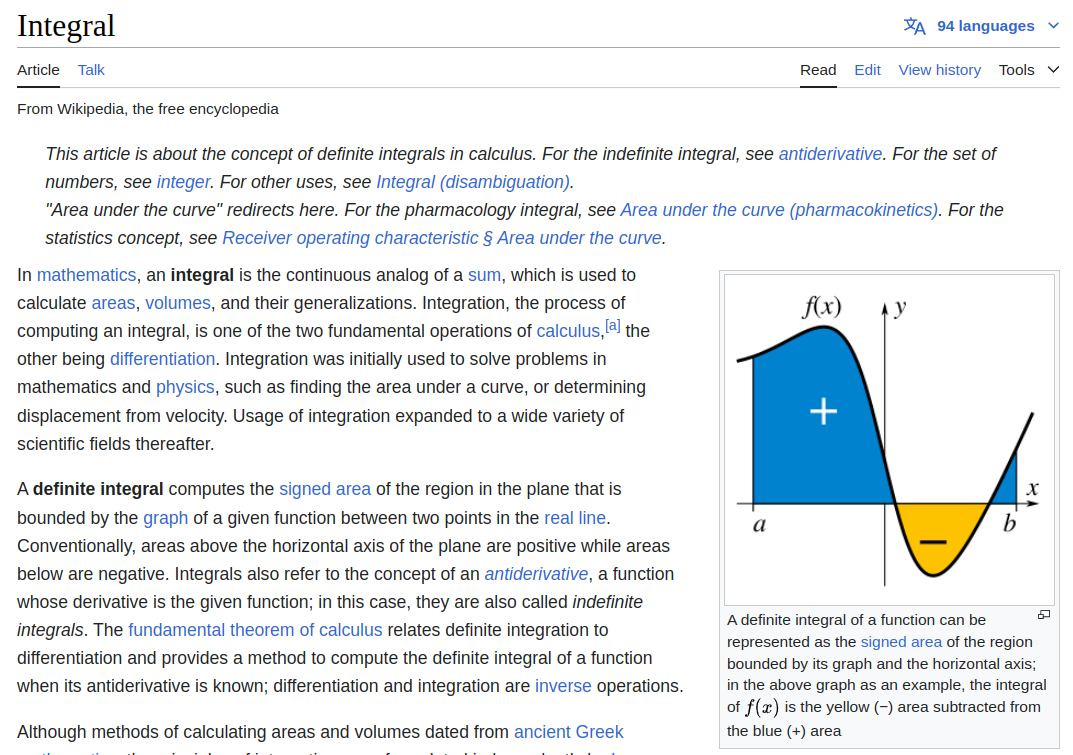
\includegraphics[width=1\linewidth]{../latex-image/linking3}
	\end{frame}
	\begin{frame}{Bi-directional Linking and Graph View}
	\centering
	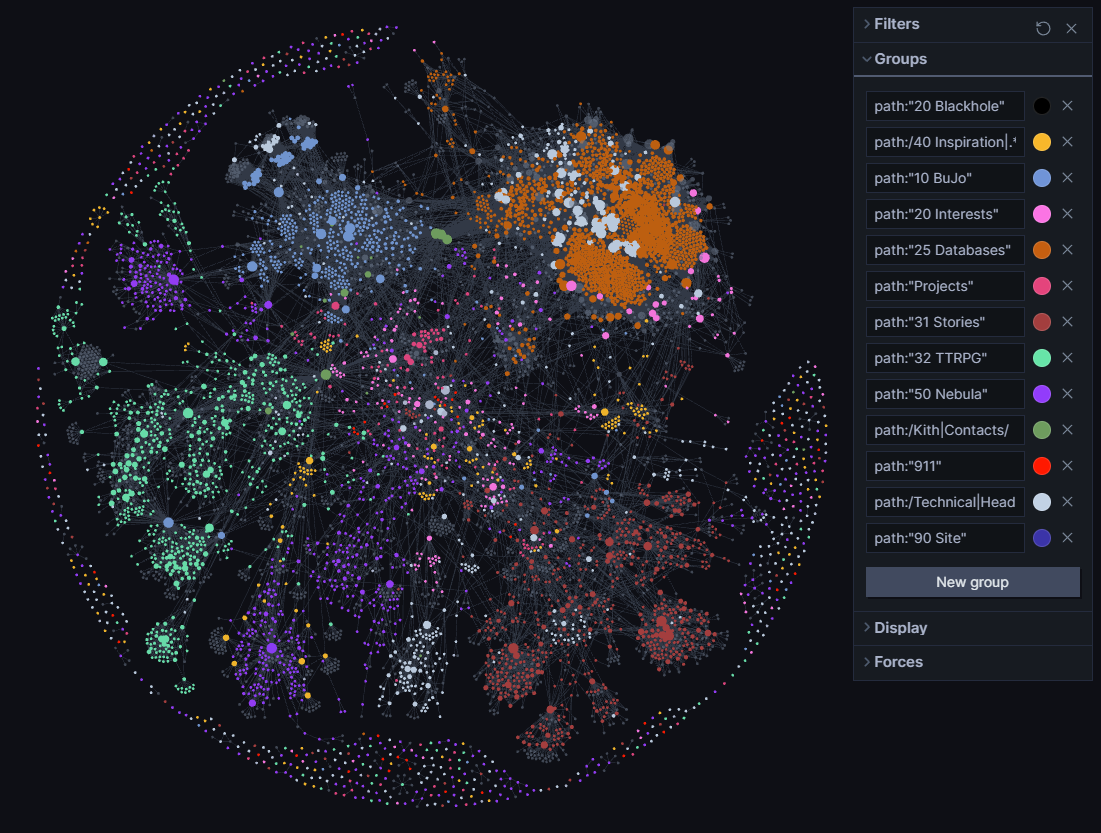
\includegraphics[width=1\linewidth]{../latex-image/graphview}
	\end{frame}
	
	\section{Canvas}
	\begin{frame}{Canvas}
		\centering
		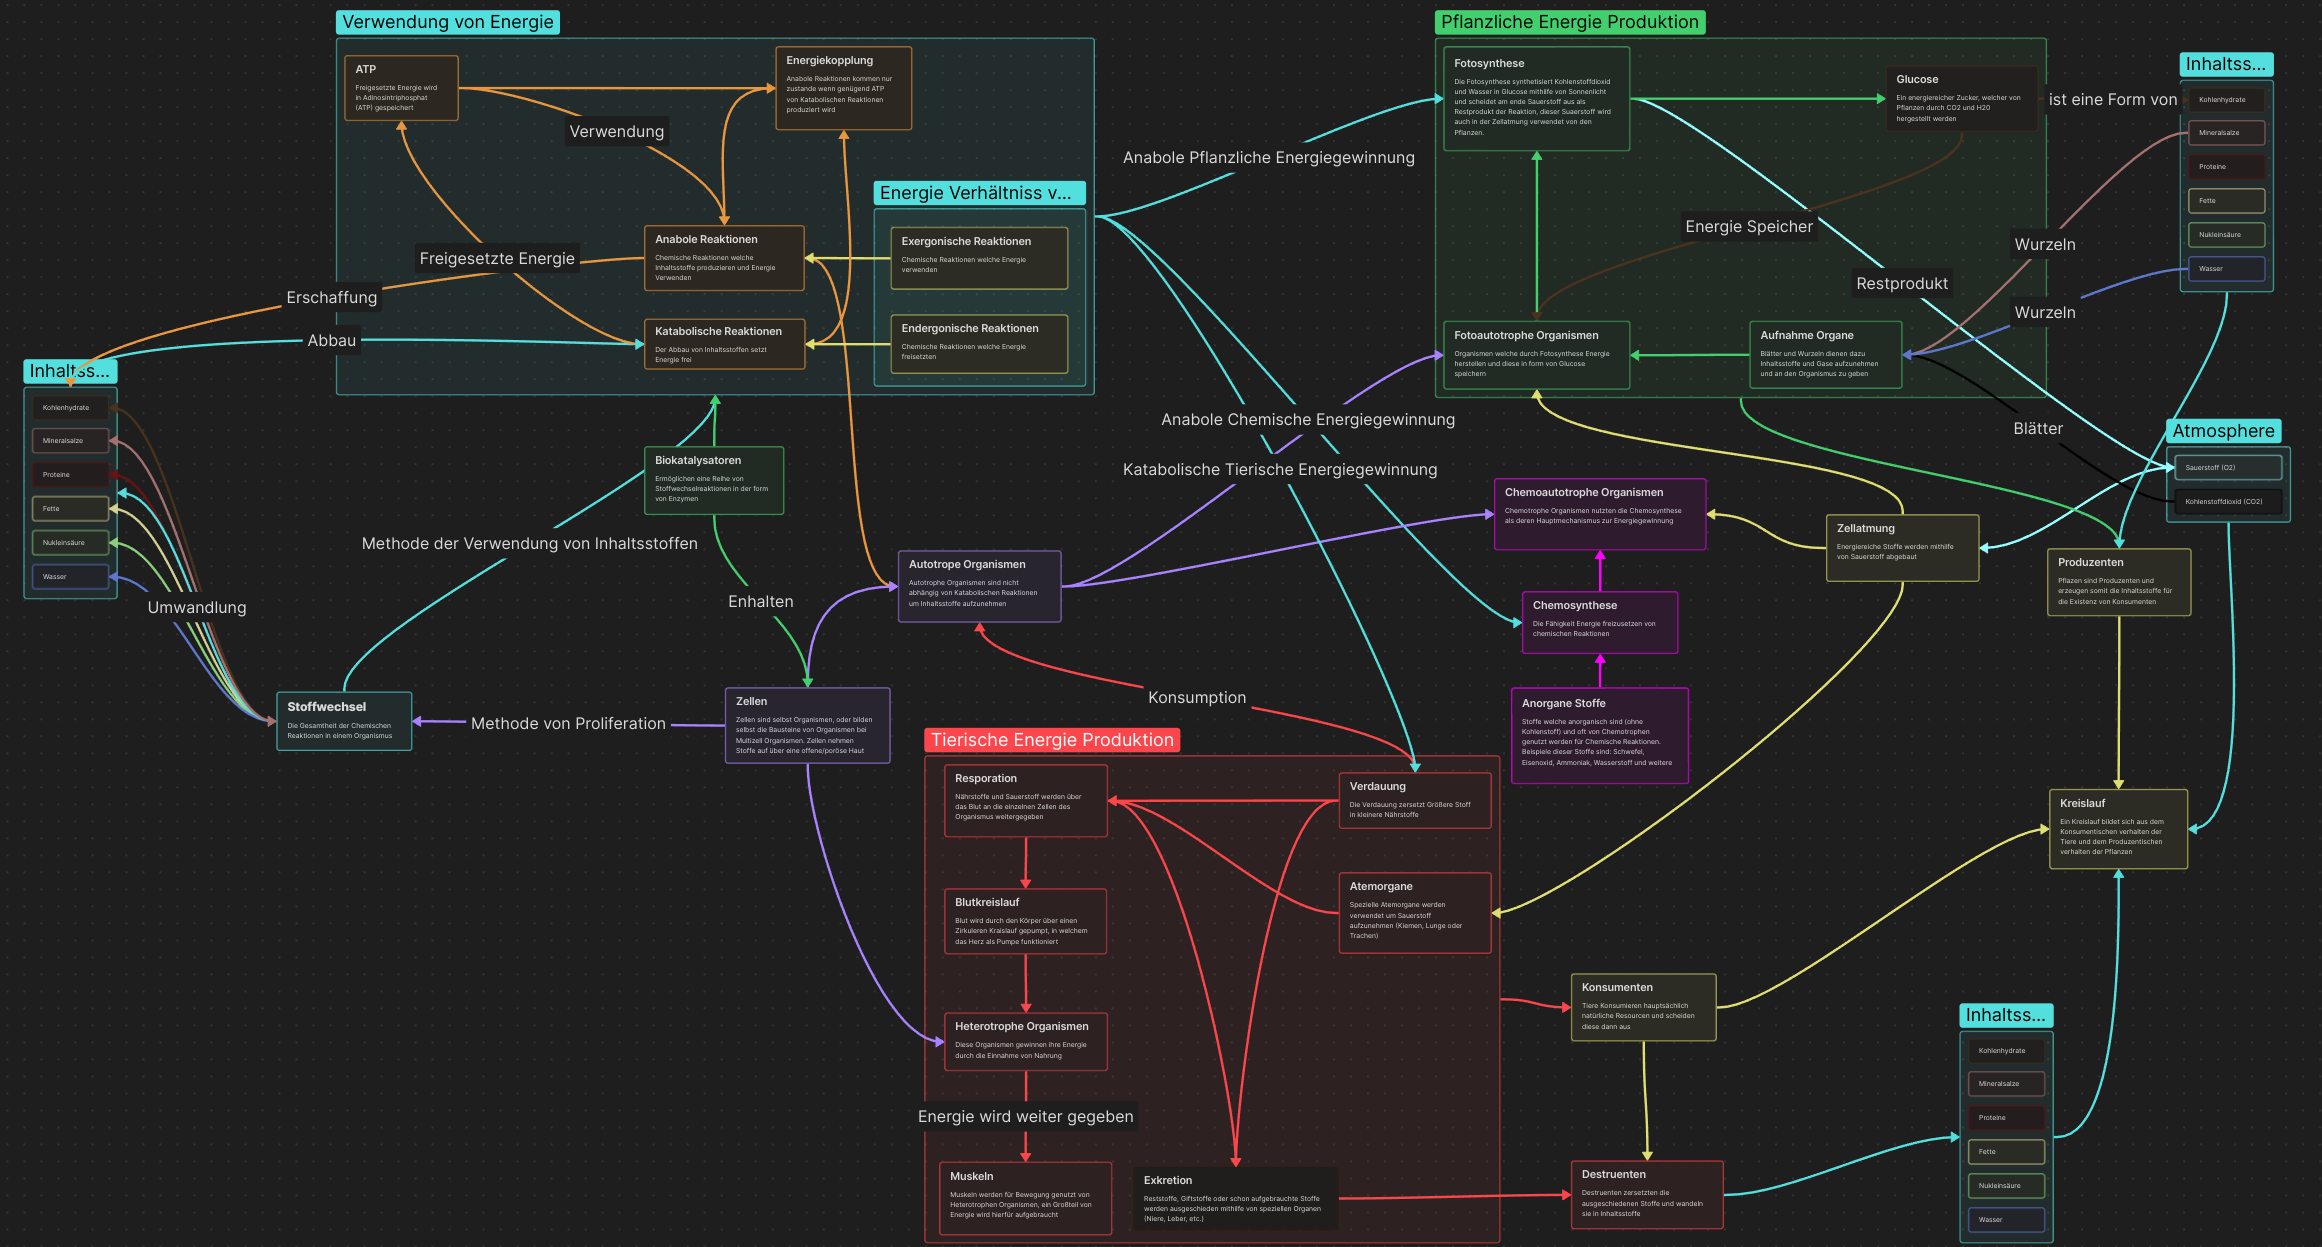
\includegraphics[scale=.185]{../latex-image/canvas1}
	\end{frame}
	\begin{frame}{Canvas}
	\centering
	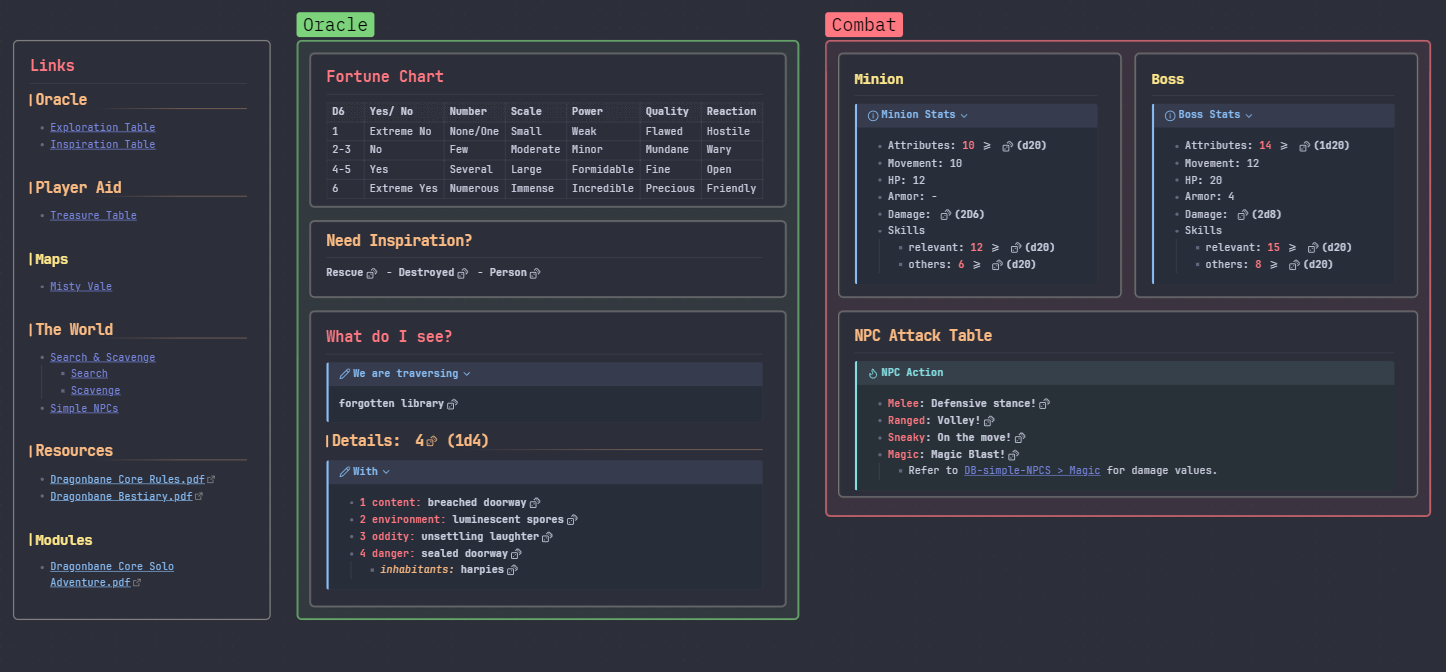
\includegraphics[scale=.3]{../latex-image/canvas2}
	\end{frame}
	\begin{frame}{Canvas}
	\centering
	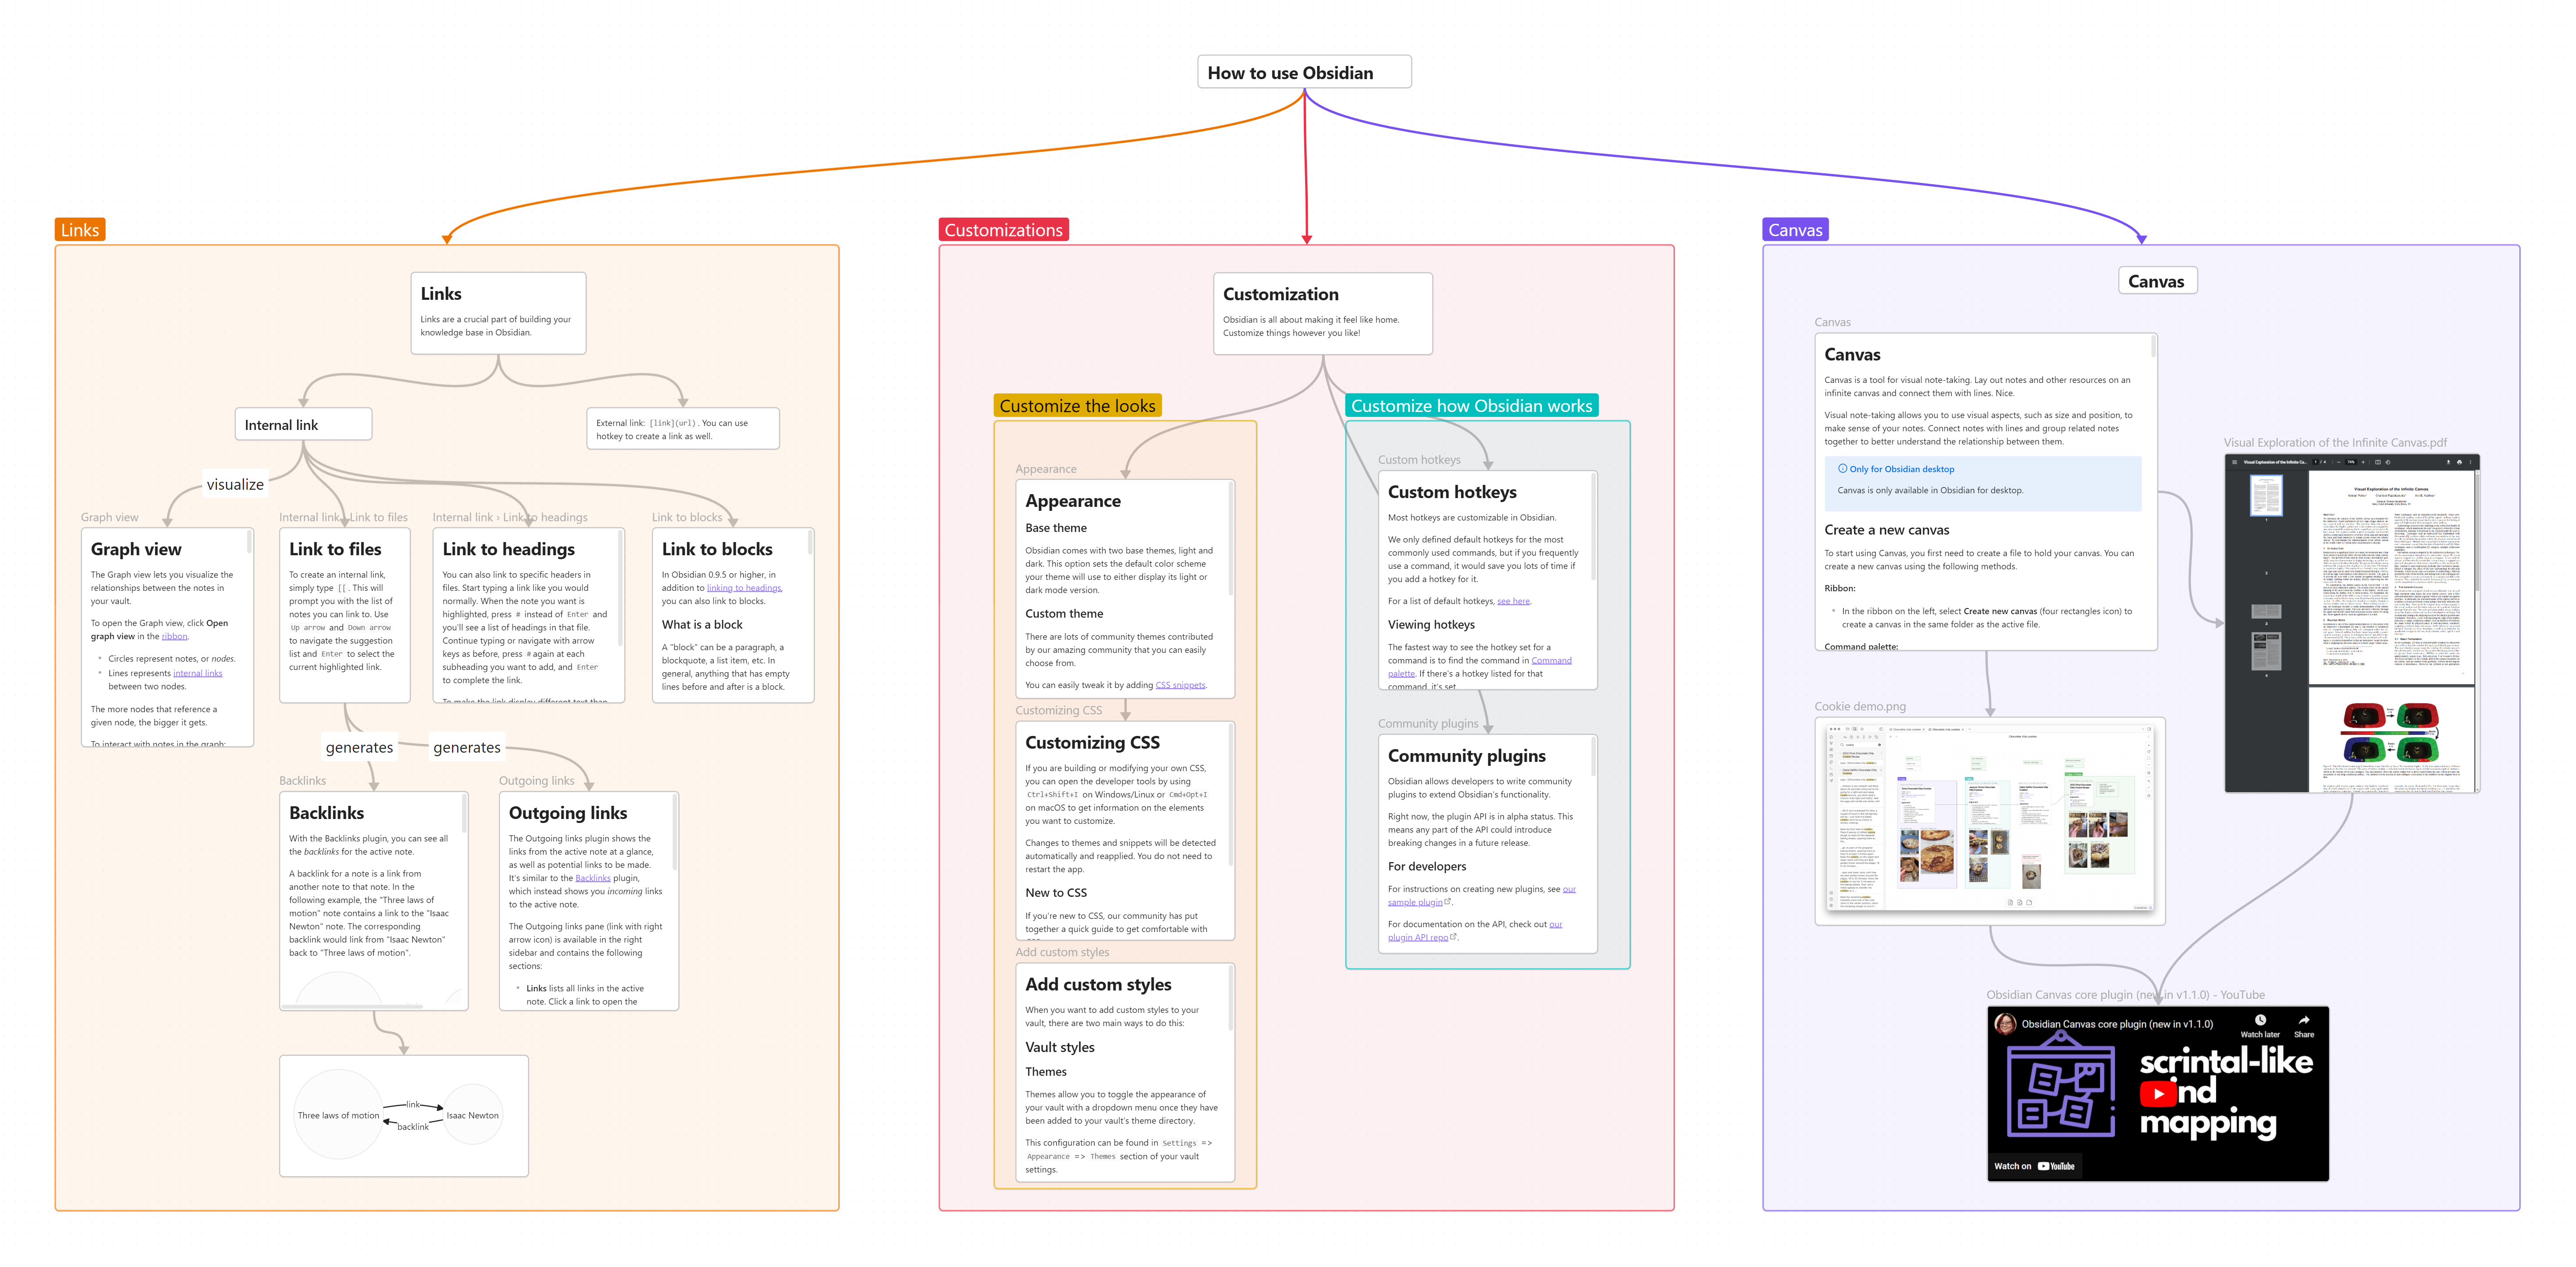
\includegraphics[scale=.055]{../latex-image/canvas3}
	\end{frame}
	
	\section{Excalidraw}
	
	\begin{frame}{Excalidraw}
		\centering
		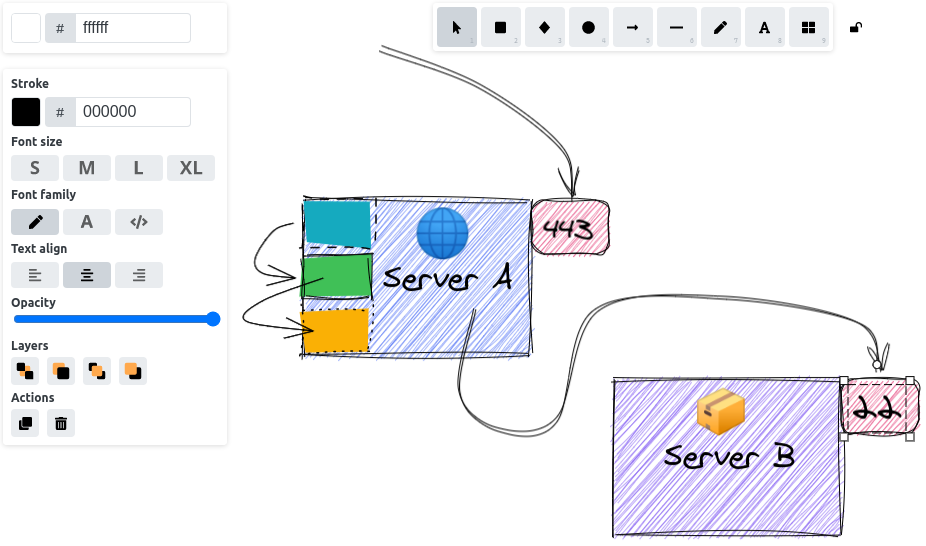
\includegraphics[width=1\linewidth]{../latex-image/excalidraw1}
	\end{frame}
	
	\begin{frame}{Excalidraw}
		\centering
		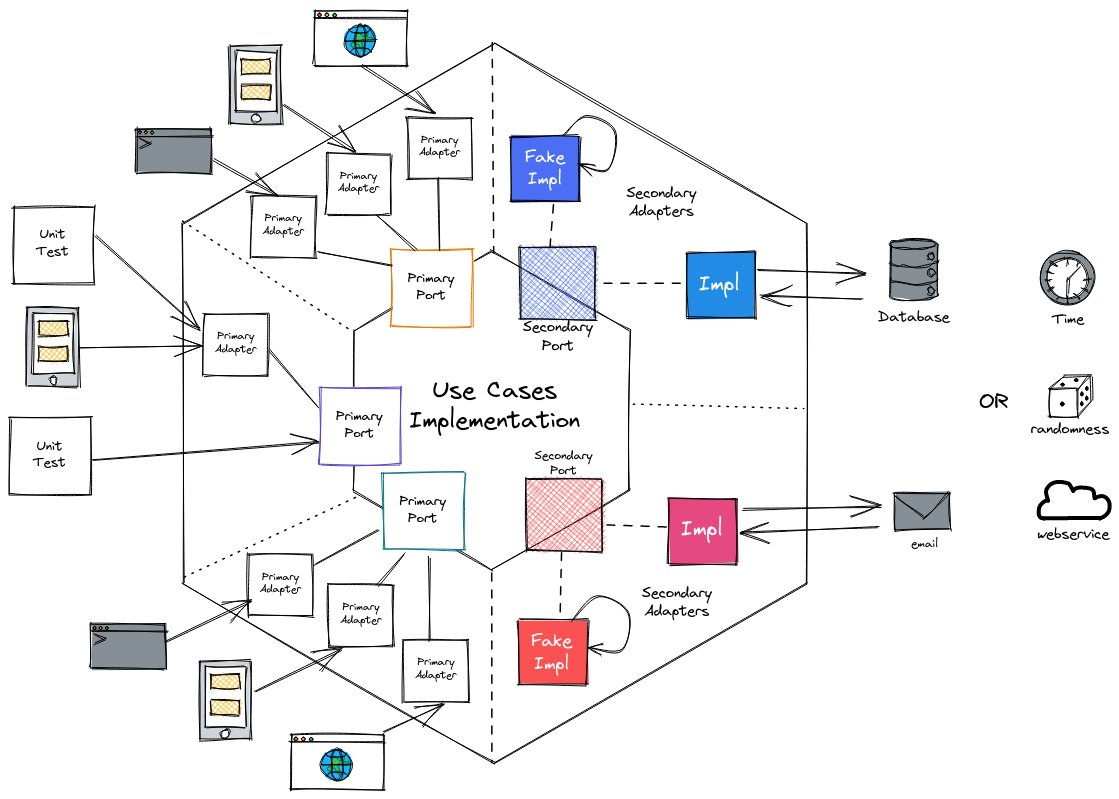
\includegraphics[width=1\linewidth]{../latex-image/excalidraw2}
	\end{frame}
	
%	% Slide 2: What is the Zettelkasten Method?
%	\section{The Zettelkasten Method}
%	\begin{frame}{What is the Zettelkasten Method?}
%		A knowledge management system developed by German sociologist Niklas Luhmann.\\
%		\vspace{0.5cm}
%		\textbf{Core Principles:}
%		\begin{itemize}
%			\item \textbf{Atomic Notes:} Each note should represent a single idea.
%			\item \textbf{Linking:} Notes are linked to other related ideas, creating a network of thoughts.
%			\item \textbf{No Hierarchies:} There’s no fixed structure, allowing organic growth of ideas.
%		\end{itemize}
%	\end{frame}
%	
%	% Slide 3: Why Combine Obsidian with Zettelkasten?
%	\begin{frame}{Why Combine Obsidian with Zettelkasten?}
%		\textbf{Obsidian's Strengths:}
%		\begin{itemize}
%			\item Excellent for implementing the Zettelkasten principle of linking notes through backlinks and forward links.
%			\item Allows notes to evolve over time, and connections can be discovered as your knowledge base grows.
%		\end{itemize}
%		\vspace{0.5cm}
%		\textbf{Zettelkasten's Strengths:}
%		\begin{itemize}
%			\item Helps in knowledge retention and creative idea development by connecting and revisiting ideas regularly.
%			\item Builds a long-term system for research and learning.
%		\end{itemize}
%	\end{frame}
%	
%	% Slide 4: How to Get Started?
%	\section{How to Get Started?}
%	\begin{frame}{How to Get Started?}
%		\begin{enumerate}
%			\item \textbf{Step 1:} Install Obsidian and create a new Vault.
%			\item \textbf{Step 2:} Write your first note as an atomic, singular idea (e.g., define a concept like “Cryptography”).
%			\item \textbf{Step 3:} Create links between notes. For example, link "Cryptography" to "Block Ciphers" by typing \texttt{[[Block Ciphers]]}.
%			\item \textbf{Step 4:} Use the Graph View to visualize how your notes are connected.
%			\item \textbf{Step 5:} Utilize tags and folders only if needed for initial organization, but rely primarily on links.
%		\end{enumerate}
%	\end{frame}
%	
%	% Slide 5: Key Plugins for Zettelkasten in Obsidian
%	\begin{frame}{Key Plugins for Zettelkasten in Obsidian}
%		\textbf{Essential Plugins:}
%		\begin{itemize}
%			\item \textbf{Graph View:} Helps visualize your network of notes.
%			\item \textbf{Dataview:} Enables you to create dynamic lists and queries from your notes (useful for tracking topics or projects).
%			\item \textbf{Backlinks:} Shows related notes, even if you haven’t manually linked them.
%			\item \textbf{Templater:} Allows you to create reusable templates for faster note creation.
%		\end{itemize}
%	\end{frame}
%	
%	% Slide 6: Closing Remarks
%	\begin{frame}{Closing Remarks}
%		\textbf{Obsidian and Zettelkasten together form a powerful, non-linear system of knowledge.}\\
%		\vspace{0.5cm}
%		\textbf{Key Advice:}
%		\begin{itemize}
%			\item Start small, with atomic notes and links.
%			\item Over time, as your notes grow, you will see the interconnected nature of your ideas, enhancing your learning and research capabilities.
%		\end{itemize}
%	\end{frame}
	
	\newpage
	{\setbeamercolor{palette primary}{fg=black, bg=-blue}
		\begin{frame}[standout]
			Questions ?\\
			\texttt{hacker3740@kookmin.ac.kr}
		\end{frame}
	}
	
	%\appendix
	%
	%\begin{frame}[fragile]{Backup slides}
	%  Sometimes, it is useful to add slides at the end of your presentation to
	%  refer to during audience questions.
	%
	%  The best way to do this is to include the \verb|appendixnumberbeamer|
	%  package in your preamble and call \verb|\appendix| before your backup slides.
	%
	%  \themename will automatically turn off slide numbering and progress bars for
	%  slides in the appendix.
	%\end{frame}
	%
	%\begin{frame}[allowframebreaks]{References}
	%
	%  \bibliography{demo}
	%  \bibliographystyl{abbrv}
	%
	%\end{frame}
	
\end{document}
